\documentclass[../main.tex]{subfiles}
\graphicspath{{\subfix{../images/}}}
\begin{document}



        \begin{figure}[hp]
          \centering
          \includegraphics[width=9cm]{MiddleEar.eps}
          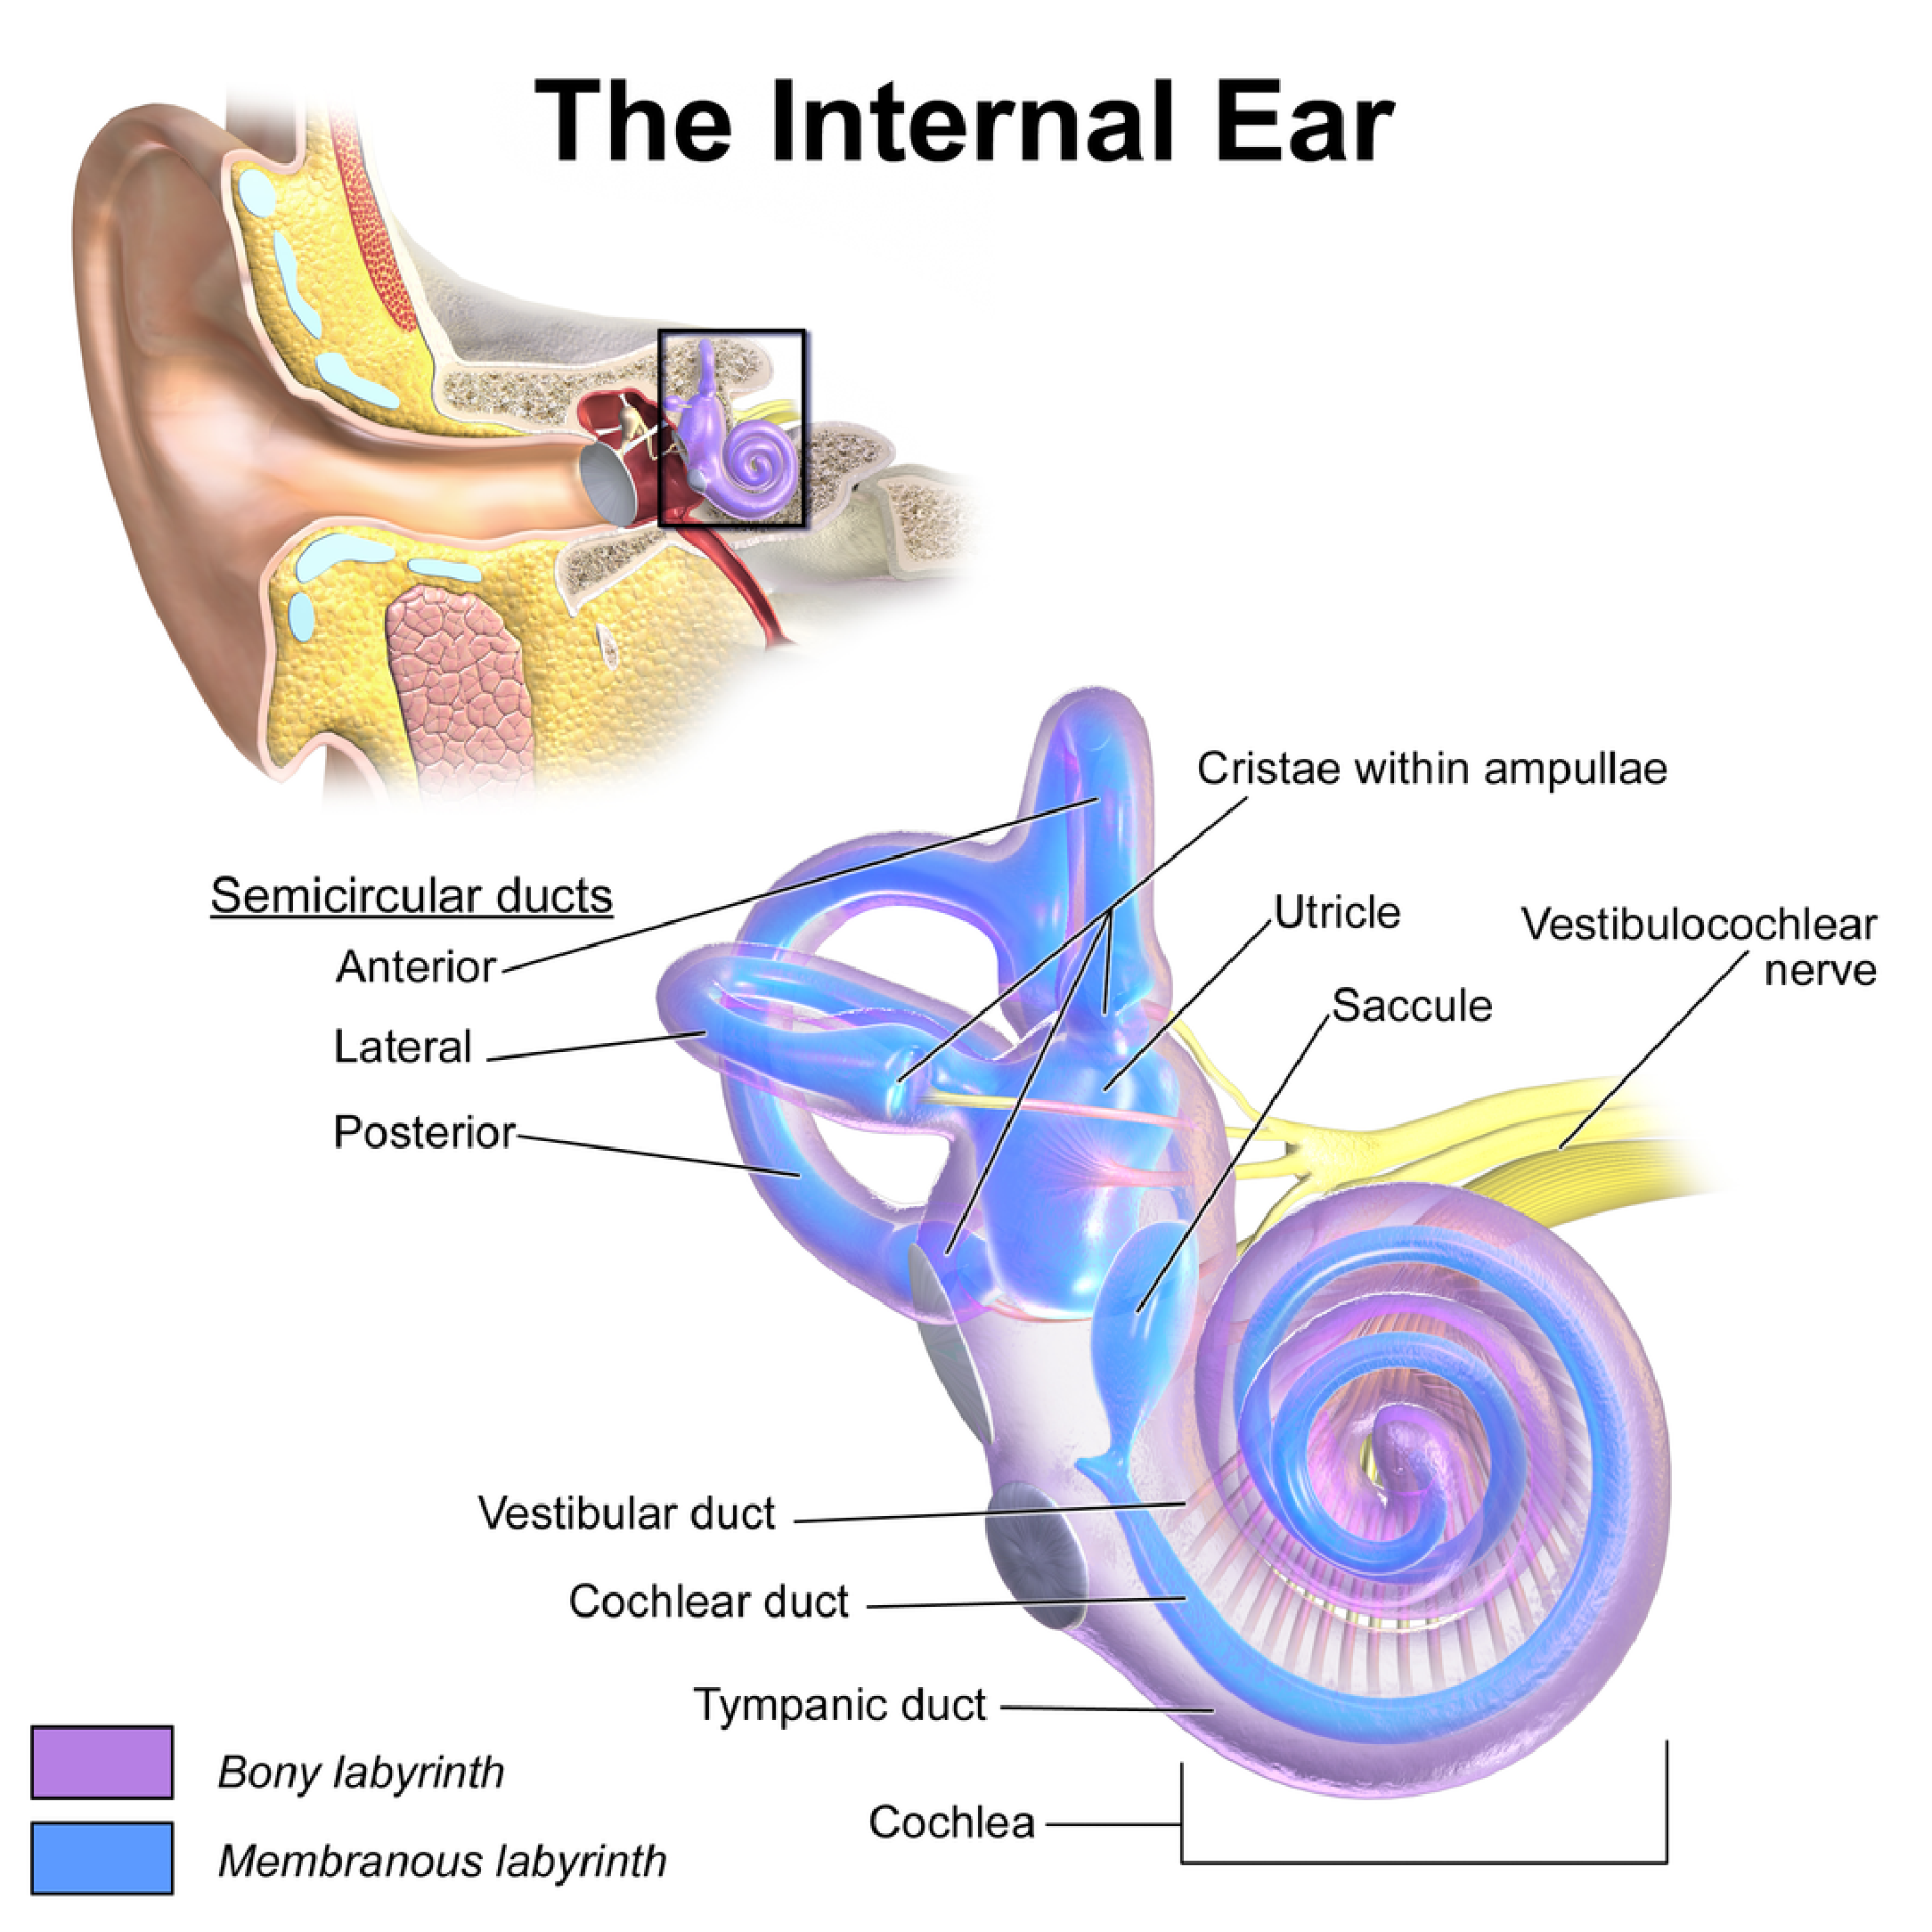
\includegraphics[width=9cm]{InternalEar.eps}
          \caption[The vestibular system]{The vestibular system~\cite{BlausenLimbic}}
        \end{figure}

        \subsubsection{The Sense of Hearing}\index{sense!hearing}

        In the inner ear, which is filled with liquid, there are about 30,000 auditory sensory cells.
        External sound waves enter through the ear canal and hit the eardrum (tympanic membrane).
        The eardrum passes the vibrations on over the little bones\footnote{auditory ossicles} hammer (malleus), anvil (incus) and the stirrup (stapes) to the internal ear.
        The vibrations also get transmitted by the skin and the skull.
        \newpage

        \subsubsection{The Sense of Balance}\index{sense!balance}

        \begin{figure}[htb]
          \centering
           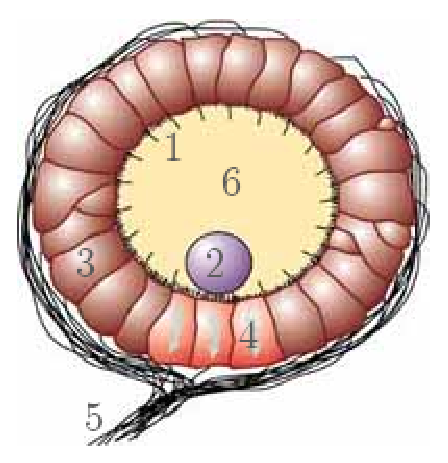
\includegraphics[width=4cm]{Statocyst.eps}
          \caption[The vestibular organ]{The vestibular organ~\cite{statolith}}
        \end{figure}

        
        We can only walk upright with the help of this sense. Their receptors sit in the vestibular organ, a part of the internal ear. Picture shows a simplified mechanism how it works.

        A calcine particle (2) is inside a hollow organ, filled with a viscous fluid (6).
        The organ is lined on the inside with sensory cells (3), which have their free nerve endings (1) inside the liquid.
        Due to gravity, it slowly sinks down and triggers (4) the sensory cells, by touching the neurons, the nerve endings.
        The collected information is then transmitted over the balance nerve (5).
        

        Drunk people have difficulties with the balance. This is due to the fact that the alcohol in the blood dehydrates the fluid inside the vestibular organ. The calcine ball moves sluggishly and being off balance only gets registered with a delay. Or it even has difficulties settling down and keeps floating, the sense of what's up and down is missing.

        When the vestibular concludes that the human is upright, it promotes alpha
        and beta waves (awake state). When it detects the human to be in a lying position it promotes delta waves (sleep) and if it detects the human to be in an inverted position (like the headstand) it promotes theta brain waves, which lead into deep meditative states and to homeostasis, the bodily equilibrium.

        Part of this calcine ball might break off and get stuck between the neurons.
        These neurons get then constantly excited. This is one possible cause of tinnitus.

        \section{Balance Training in Daily Life}

        Make your phone call or brush your teeth standing on one leg, or practice the headstand over your lunch break.
        Maybe you feel like learning to ride a unicycle or balance over a fallen tree on your walk.
        Always stay in motion and find this way your inner and outer balance and equilibrium.

        \epigraph{Seek the peace and calmth by the means of balance, not by ceasing your actions.}{\textit{Friedrich Schiller}}
        
      \end{document}